%\iffalse
\let\negmedspace\undefined
\let\negthickspace\undefined
\documentclass[journal,12pt,twocolumn]{IEEEtran}
\usepackage{cite}
\usepackage{amsmath,amssymb,amsfonts,amsthm}
\usepackage{algorithmic}
\usepackage{graphicx}
\usepackage{textcomp}
\usepackage{xcolor}
\usepackage{txfonts}
\usepackage{listings}
\usepackage{enumitem}
\usepackage{mathtools}
\usepackage{gensymb}
\usepackage{comment}
\usepackage[breaklinks=true]{hyperref}
\usepackage{tkz-euclide} 
\usepackage{listings}
\usepackage{gvv}                            \usepackage{tikz}
\usepackage{circuitikz}
\def\inputGnumericTable{}                                
\usepackage[latin1]{inputenc}                            
\usepackage{color}                                       
\usepackage{array}                                       
\usepackage{longtable}                                   
\usepackage{calc}                              
\usepackage{tikz}
\usepackage{multirow}                                    
\usepackage{hhline}                                      
\usepackage{ifthen}                            
\usepackage{caption}
\usepackage{lscape}
\usepackage{amsmath}
\newtheorem{theorem}{Theorem}[section]
\newtheorem{problem}{Problem}
\newtheorem{proposition}{Proposition}[section]
\newtheorem{lemma}{Lemma}[section]
\newtheorem{corollary}[theorem]{Corollary}
\newtheorem{example}{Example}[section]
\newtheorem{definition}[problem]{Definition}
\newcommand{\BEQA}{\begin{eqnarray}}
\newcommand{\EEQA}{\end{eqnarray}}
\newcommand{\define}{\stackrel{\triangle}{=}}
\theoremstyle{remark}
\newtheorem{rem}{Remark}

\begin{document}

\bibliographystyle{IEEEtran}
\vspace{3cm}

\title{GATE 2021 CH Q52}
\author{EE23BTECH11009 - AROSHISH PRADHAN$^{*}$% <-this % stops a space
}
\maketitle
\newpage
\bigskip
\textbf{Question:} A system has a transfer function
\begin{align}
    G(s) = \frac{3e^{-4s}}{12s + 1}\nonumber
\end{align}
When a step-change of magnitude $M$ is given to the system input, the final value of the system output is measured to be 120. The value of M is \_\_\_\_\_.
\hfill(GATE 2021 CH Q52)\\
\solution
\begin{table}[!h]
    \centering
    \begin{tabular}{|c|c|c|}
    \hline
       \textbf{Symbol}  & \textbf{Value} &  \textbf{Description}\\
    \hline
       $V_{in}$  &  &  Input Voltage\\
    \hline
        $V_{out}$ & & Output Voltage\\
    \hline
        $f$ & $1000Hz$ & Input Wave Frequency\\
    \hline
        $T$ & $\dfrac{1}{f} = 10^{-3} s$ & Input Wave Time Period\\
    \hline
        \multirow{4}{*}{$R$} & (a) $0.5k\Omega$ & \multirow{4}{*}{Resistance}\\
        \cline{2-2}
        & (b) $5k\Omega$ &\\
        \cline{2-2}
        & (c) $0.5k\Omega$ &\\
        \cline{2-2}
        & (d) $5k\Omega$ &\\
    \hline
        \multirow{4}{*}{$C$} & (a) $0.1\mu F$ & \multirow{4}{*}{Capacitance}\\
        \cline{2-2}
        & (b) $1\mu F$ &\\
        \cline{2-2}
        & (c) $0.1\mu F$ &\\
        \cline{2-2}
        & (d) $1\mu F$ &\\
    \hline
        $\tau$ & $RC$ & Time Constant\\
    \hline
    \end{tabular}
    \caption{Given Parameters}
    \label{tab:1_gate.23.ph.37}
\end{table}


Given, input step-change:
\begin{align}
    x(t) &= Mu(t)\\
    u(t) &\system{L} \frac{1}{s}\\
    \implies X(s) &= \frac{M}{s}
\end{align}
Transfer Function:
\begin{align}
    G(s) &= \frac{Y(s)}{X(s)} = \frac{3e^{-4s}}{12s + 1}\\
    \implies Y(s) &= \frac{3e^{-4s}}{12s + 1}\frac{M}{s}
\end{align}
$\therefore$ system output
\begin{align}
     \lim_{s\rightarrow0}sY(s) &= 120\\
    \implies \lim_{s\rightarrow0}\brak{\frac{3e^{-4s}}{12s + 1}M} &= 120\\
    \implies 3M &= 120\\
    \implies M &= 40
\end{align}

\begin{figure}
    \centering
    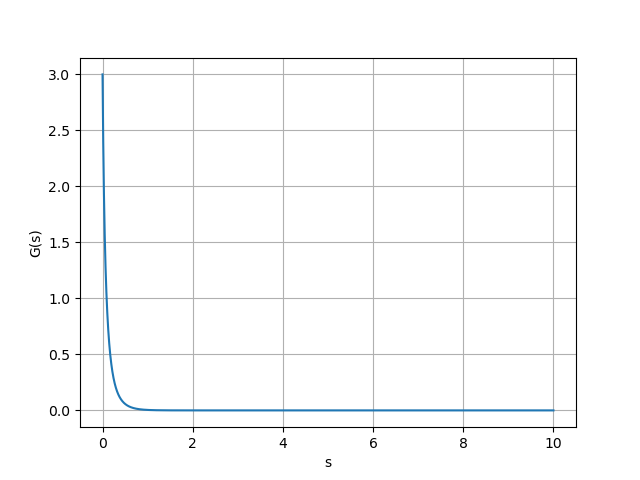
\includegraphics[width = \columnwidth]{figs/assign9.png}
    \caption{Plot of $\abs{G(j\omega)}$} vs $\omega$
    \label{fig:1_gate.21.ch.52}
\end{figure}
\end{document}
